\documentclass{article}
\usepackage{arxiv}

\usepackage{XCharter}
\usepackage[T2A]{fontenc}
\usepackage[utf8]{inputenc}
\usepackage[russian,english]{babel}

\usepackage{url}
\usepackage{booktabs}
\usepackage{amsfonts}
\usepackage{nicefrac}
\usepackage{microtype}
\usepackage{lipsum}
\usepackage{graphicx}
\usepackage[numbers]{natbib}  % Change 'authoryear' to 'numbers'
\usepackage{doi}


\title{Face-aware Arbitrary Image Style Transfer}

\author{ Karatyshchev~Dmitry\thanks{GitHub: https://github.com/dmforit/style-transfer-mode} \\
	Lomonosov Moscow State University\\
	\texttt{dmitrykaratyshchev@gmail.com} \\
	%% examples of more authors
	\And
	Viktor~Kitov \thanks{Web Page: https://victorkitov.github.io} \\
	Lomonosov Moscow State University,\\
	Plekhanov Russian University of Economics\\
	\texttt{v.v.kitov@yandex.ru} \\
}
\date{}

%%% Add PDF metadata to help others organize their library
%%% Once the PDF is generated, you can check the metadata with
%%% $ pdfinfo template.pdf
\hypersetup{
pdftitle={Face-aware Arbitrary Image Style Transfer},
pdfsubject={cs.CV, cs.LG, eess.IV, },
pdfauthor={Karatyshchev~Dmitry, Viktor~Kitov},
pdfkeywords={Image style transfer, Image processing},
}

\begin{document}
\maketitle

\begin{abstract}
Arbitrary style transfer techniques have achieved significant results in machine learning, enabling the transformation of input images into artistic outputs while preserving content structures. Although existing methods for style transfer address the challenge of preserving facial details during stylization, they often suffer from noticeable artifacts and fail to maintain identity consistency. Recent advancements, such as RAST (Restorable Arbitrary Style Transfer), have addressed the challenge of maintaining high-fidelity restorability during style transfer by integrating multi-restoration processes. Building upon the foundational improvements introduced by RAST, our work introduces a novel framework for Face-aware Arbitrary Image Style Transfer that specifically enhances the handling of facial regions. Recognizing that existing methods often fail to preserve the details and identity of faces, we propose an architecture that incorporates adaptive facial region detection and targeted feature modulation to maintain facial consistency while applying stylistic transformations. This improvement ensures that essential facial features, such as expressions and identity markers, remain recognizable and coherent in the stylized output. Extensive experiments demonstrate that our enhanced model not only preserves global and local content better but also significantly outperforms baseline methods in perceptual quality, particularly in human-centric images. This work paves the way for more refined and identity-preserving artistic transformations, bridging the gap between arbitrary style transfer and realistic face representation.
\end{abstract}

\keywords{Image style transfer \and Image processing}

\section{Introduction}
\label{sec:introduction}

In recent years, arbitrary style transfer has emerged as a powerful tool in the realm of computer vision and machine learning, enabling the transformation of images into various artistic styles while preserving the underlying content structure. This capability has opened up numerous applications, from digital art creation to enhancing visual effects in multimedia. However, despite the impressive progress in arbitrary style transfer, one of the most challenging aspects remains the preservation of facial details and identity consistency during stylization. Faces, being highly sensitive and complex structures, often suffer from artifacts and distortions that undermine the realism and integrity of the transformed images.

The development of arbitrary style transfer has its roots in early attempts to separate image content and style, drawing inspiration from the field of neuroscience. The foundational work by Gatys et al. \cite{gatys2015neural} in 2015 introduced the concept of using convolutional neural networks (CNNs) to achieve style transfer by optimizing images to match both content and style representations learned from deep layers of pre-trained networks. This breakthrough demonstrated that complex visual patterns could be transferred between images, sparking a surge of interest in the field.

Subsequent methods sought to address limitations such as computational inefficiency and the restriction to a limited set of styles. Techniques like Fast Neural Style Transfer, proposed by Johnson et al., used feed-forward neural networks to achieve real-time stylization \cite{johnson2016perceptual, li2017universal}, enabling broader applications. The evolution continued with the introduction of universal style transfer approaches, allowing arbitrary styles to be applied without the need for per-style retraining. These approaches laid the groundwork for more sophisticated methods that improved adaptability and efficiency.

Recent advancements have focused on enhancing the quality and versatility of arbitrary style transfer, including methods that prioritize maintaining structural coherence and integrating multi-level feature transformations. Despite these advances, preserving facial identity during stylization remained a persistent challenge, prompting further exploration and innovation in face-aware algorithms.

Existing methodologies have attempted to address these challenges with varying degrees of success. While some approaches integrate specific constraints or additional processes to maintain facial features, they frequently encounter trade-offs that compromise either the quality of the stylization or the fidelity of the facial identity. Recent innovations, such as the Restorable Arbitrary Style Transfer (RAST) framework \cite{Ma_2023_WACV}, have shown that multi-restoration techniques can enhance the overall quality of style transfer, ensuring that critical content can be restored after the stylization process. Yet, even these advanced methods fall short when applied to images where facial detail is paramount, leading to outputs that may lack the nuance necessary for identity preservation.

To bridge this gap, our work presents a novel framework specifically designed for Face-aware Arbitrary Image Style Transfer. This framework incorporates adaptive facial region detection and targeted feature modulation, enhancing the capacity to preserve facial identity and expression integrity throughout the stylization process. By prioritizing the accurate representation of facial features and identity markers, our method ensures that the stylized output remains coherent and recognizable, even in highly stylized transformations. Our extensive experiments validate that this approach not only maintains global and local content but also delivers superior perceptual quality compared to existing state-of-the-art methods, particularly in scenarios involving human-centric imagery. This advancement sets a new benchmark for identity-preserving style transfer and paves the way for more realistic and expressive artistic transformations.




\section{Related work}
\label{sec:related_work}

\lipsum[4] See Section \ref{sec:related_work}.

\subsection{Headings: second level}
\lipsum[5]
\begin{equation}
	\xi _{ij}(t)=P(x_{t}=i,x_{t+1}=j|y,v,w;\theta)= {\frac {\alpha _{i}(t)a^{w_t}_{ij}\beta _{j}(t+1)b^{v_{t+1}}_{j}(y_{t+1})}{\sum _{i=1}^{N} \sum _{j=1}^{N} \alpha _{i}(t)a^{w_t}_{ij}\beta _{j}(t+1)b^{v_{t+1}}_{j}(y_{t+1})}}
\end{equation}

\section{Proposed method}
\label{sec:proposed_method}
% \subsubsection{Headings: third level}
\lipsum[6]

% \paragraph{Paragraph}
% \lipsum[7]

\section{Experimental results}
\label{sec:experiments}

\lipsum[20]

\section{Conclusion}
\label{sec:conclusion}

\lipsum[21]

% \subsection{Citations}
% Citations use \verb+natbib+. The documentation may be found at
% \begin{center}
% 	\url{http://mirrors.ctan.org/macros/latex/contrib/natbib/natnotes.pdf}
% \end{center}

% Some people thought a thing \cite{kour2014real, hadash2018estimate} but other people thought something else \cite{kour2014fast}. Many people have speculated that if we knew exactly why \cite{kour2014fast} thought this\dots

% \subsection{Figures}
% \lipsum[10]
% See Figure \ref{fig:fig1}. Here is how you add footnotes. \footnote{Sample of the first footnote.}
% \lipsum[11]

% \begin{figure}
% 	\centering
% 	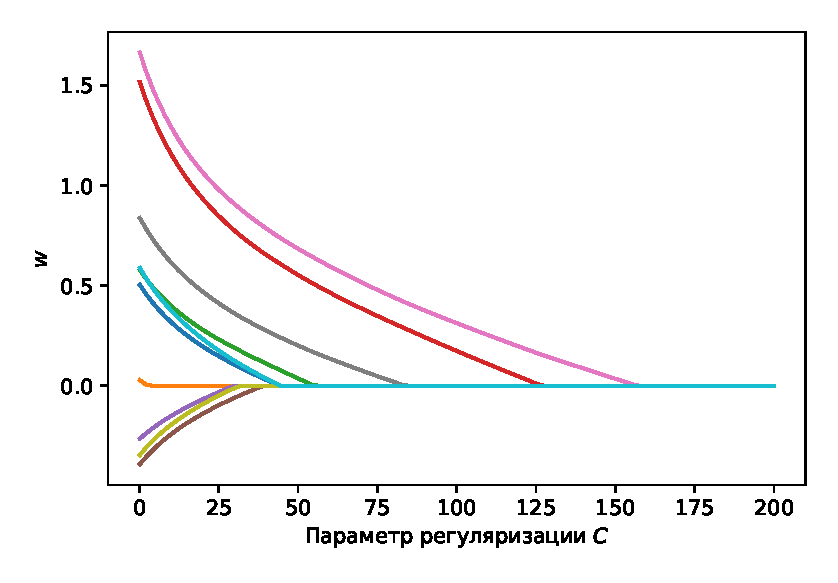
\includegraphics[width=0.5\textwidth]{figures/log_reg_cs_exp.eps}
% 	\caption{Sample figure caption.}
% 	\label{fig:fig1}
% \end{figure}

% \subsection{Tables}
% See awesome Table~\ref{tab:table}.

% The documentation for \verb+booktabs+ (`Publication quality tables in LaTeX') is available from:
% \begin{center}
% 	\url{https://www.ctan.org/pkg/booktabs}
% \end{center}


% \begin{table}
% 	\caption{Sample table title}
% 	\centering
% 	\begin{tabular}{lll}
% 		\toprule
% 		\multicolumn{2}{c}{Part}                   \\
% 		\cmidrule(r){1-2}
% 		Name     & Description     & Size ($\mu$m) \\
% 		\midrule
% 		Dendrite & Input terminal  & $\sim$100     \\
% 		Axon     & Output terminal & $\sim$10      \\
% 		Soma     & Cell body       & up to $10^6$  \\
% 		\bottomrule
% 	\end{tabular}
% 	\label{tab:table}
% \end{table}

% \subsection{Lists}
% \begin{itemize}
% 	\item Lorem ipsum dolor sit amet
% 	\item consectetur adipiscing elit.
% 	\item Aliquam dignissim blandit est, in dictum tortor gravida eget. In ac rutrum magna.
% \end{itemize}


\bibliographystyle{unsrt}  % Keeps the references in order of appearance
\bibliography{references}

\end{document}